\documentclass[10pt]{article}
\textwidth 16.5cm
\textheight 23.5cm
\oddsidemargin 0pt
\topmargin -2cm
% \usepackage{epsf}

% Draft watermark
% \usepackage{draftwatermark}

% Font and formatting
\usepackage[default]{lato}
\usepackage[skip=3pt]{parskip}
\usepackage{titlesec}
\titlespacing{\paragraph}{0pt}{*1}{*2}

% \usepackage[compact]{titlesec} 


% Writing maths
\usepackage{
    amsmath, % aligns, equations, etc.
    amsfonts, % blackboard bold, etc.
    bbm, % blackboard bold for numbers.
}

% Figures
\usepackage{graphicx}

% References
\usepackage[colorlinks,linkcolor=black,citecolor=blue,urlcolor=blue,breaklinks = true]{hyperref}
\usepackage[sort&compress, numbers]{natbib}
\bibliographystyle{unsrtnat}
% \setcitestyle{authoryear, open={(},close={)}}


% Acronyms
\usepackage[acronym, toc]{glossaries-extra}

\setabbreviationstyle[acronym]{long-short}
\glssetcategoryattribute{acronym}{nohyperfirst}{true}
\renewcommand*{\glsdonohyperlink}[2]{%
 {\glsxtrprotectlinks \glsdohypertarget{#1}{#2}}}

 \newacronym{bfo}{BFO}{Border Force Officer}
 \newacronym[plural=SLAs, firstplural=Service Level Agreements]{sla}{SLA}{Service Level Agreement}
 \newacronym[plural=eGates, firstplural=electronic passport Gates]{egate}{eGate}{electronic passport Gate}
 \newacronym[plural=KPIs, firstplural=Key Performance Indicators]{kpi}{KPI}{Key Performance Indicator}

% Inline comments from Jacob and Bella
\usepackage{xcolor}
\usepackage[draft,inline,nomargin,index]{fixme}
\fxsetup{theme=color,mode=multiuser}
\FXRegisterAuthor{jb}{ajb}{\color{blue} JB}
\FXRegisterAuthor{bd}{abd}{\color{red} BD}

\title{Anticipating Demand on Immigration at Edinburgh Airport}
% Planning for future immigration demand at Edinburgh Airport
% Simulations of Immigration Queues at Edinburgh Airport: Report}
 \author{Isabella Deutsch and Jacob R. Bradley}
 % \\ \emph{School of Mathematics, University of Edinburgh}}
 \date{}

\begin{document}
\maketitle

\section{Introduction}

A large number of passengers arriving internationally at Edinburgh Airport need to pass through immigration. These passengers are either processed at a desk staffed by a \gls{bfo} or, for passengers of certain nationalities, at an automated \gls{egate}. With overall passenger footfall expected to increase substantially over the next five years, pressure on immigration services is also growing, and the airport will need to adapt its operations in order to accommodate its international arrivals safely and efficiently. In particular, the airport has committed to several \glspl{sla} ensuring quality of experience for arrivals. \bdnote{Need to define the SLA clearly below for this to make sense.} One avenue being explored to meet \glspl{sla} under increased demand is the expanded use of \glspl{egate}, both through additional construction and measures encouraging increased uptake \cite{UK_border_2025}. In this report we investigate the outcomes of these measures, providing clear recommendations for \gls{egate} construction and usage over the next five years (2023-2027). For key results, see our one page high-level summary.
% This does not apply for anyone arriving from the United Kingdom (including Northern Ireland), the Crown Dependencies, and the Republic of Ireland, as there are no routine passport controls between these countries \cite{common_travel_area}.
% Only passengers of certain nationality are eligible to use the \glspl{egate}, as defined below. There are currently 9 desks and 10 \glspl{egate} in operation at Edinburgh Airport. 

\subsection{Problem Statement}
The task set by Edinburgh Airport is to develop a simulation model of immigration queuing that can be used to test a variety of demand scenarios, including overall and demographic changes in passenger arrivals, process enhancements, and increased \gls{egate} availability. 
Additionally, sensitivity analysis is required to assess the robustness of these recommendations under a variety of perturbation scenarios.
The overall performance of Edinburgh Airport's immigration queuing operation is measured via three \glspl{kpi}, defined below.

\subsection{Key Performance Indicators}

Three \glspl{kpi} have been identified to form the basis of the airport's \glspl{sla}. We define them as follows.

\begin{itemize}
    \item \textbf{Queue length(s)}: The number of passengers queuing for a desk or \gls{egate} in the immigration hall/overflow zone at any given time.
    % We report the mean, median, 75\% quantile, and maximum. This is considered for both desk and \gls{egate}-specific queues.
    \item \textbf{Queue time}: Minutes between arrival at the immigration hall/overflow zone and arrival at a desk/\gls{egate} for a given passenger arriving at Edinburgh Airport. 
    % We report the mean, median, 75\% quantile, and maximum. 
    % This are calculated both for the total of the immigration queue, as well as the desk and \gls{egate} queues separately.
    \item \textbf{Overflow usage}: The proportion of a given day for which immigration hall overflow capacity was in use.
\end{itemize}

Note that \textit{queue length} is measured as a function over time, i.e. we record the queue length every minute, even if no passengers are arriving. Based on this granular data we can then compute average and maxima statistics. The \textit{queue time}, however, is measured for each arriving passenger and we calculate averages over the passengers. The relationship between queue length and \textit{overflow usage} may be determined in part by the physical division of the immigration hall into desk and \gls{egate} queueing regions.

\subsection{Service Level Agreements}


\section{Data}
This section outlines the datasets used throughout this report. The majority of the data used for the core components of our analysis were provided by Edinburgh Airport via the Edinburgh SIAM \& IMA Student Chapter Modelling Competition \cite{modelling_competition}. Occasionally, it has been useful to make use of some external datasets, which have also been described here. These are all either in the public domain, or are accessible to all researchers participating in the modelling competition. 

\subsection{Competition Data}

We first outline the data received through the modelling competition. This data, informed by real arrivals data at Edinburgh Airport, is intended to provide a baseline set of assumptions for the composition of airport arrivals across five busy future weeks, each in early July of the years 2023-2027 respectively.
% While these represent realistic values, we are aware that they may contain approximations and/or simulated data. 
% Most notably, the arrivals data in Section~\ref{XX} is a fictitious arrivals schedule for five weeks in the future, in namely 2023 to 2027. 

\subsubsection{Operational Data}

\paragraph{Hall Capacity}
The immigration hall at Edinburgh Airport has a \textit{initial capacity} of 500 people. Its \textit{overflow capacity}, which can be used without overly impacting other areas of the operation, is a further 150 people. There is also a \textit{contingency capacity} for additional 600 people. However, its usage negatively impacts the operations of the airport.

\paragraph{Coached vs. Contact}
Once an aircraft has reached its parking position there are two ways for passengers to reach the terminal building. \textit{Contact} passengers walk by foot to the immigration queue. \textit{Coached} passengers exit the aircraft via stairs and are loaded onto buses, which bring them to the terminal building. The percentage of contact passengers lies around 80\% and varies across years.

\paragraph{eGate Eligibility for EU+ Passengers}
Passengers of the following nationalities are allowed to use \glspl{egate}: EU countries, Australia, Canada, Iceland, Japan, Liechtenstein, New Zealand, Norway, Singapore, South Korea, Switzerland, and the USA. In the following we refer to these countries as \textit{EU+}. 

\paragraph{Domestic and UK+ Flights} Flights arriving from the United Kingdom (including Northern Ireland), the Crown Dependencies, and the Republic of Ireland (referred throughout as \textit{UK+}) do not need to be processed by immigration services, as there are currently no routine passport controls between these countries \cite{common_travel_area}.

\paragraph{Early and Delayed Flights}
In the summer of 2019 only 58\% of flights arrived on time (measured if arrived within 15 minutes of scheduled arrival), 21\% were late, and 21\% were early. Of those that were early, average arrival time was 21 minutes ahead of schedule (standard deviation 6 minutes). For late arrivals, average delay was 50 minutes (standard deviation 56 minutes).

\subsubsection{Future Arrivals Data} \label{sec:future_arrivals_data}
Via the modelling competition, we have been provided with an anticipated future arrivals schedule and passenger counts for five July weeks (each Monday to Sunday) over the next five years (2023-2027). These comprise a total of 4,123 flights and represent increasing aircraft arrivals over time (Table~\ref{tab:future_arrivals_overview}). These are reflected in an increased passenger throughput over the same time period, comprising increases in both coached and contact arrivals (Figure~\ref{fig:future_passenger_burden}).
\begin{table}[!ht]
\caption{Anticipated flight schedule, 2023-2027.}
\label{tab:future_arrivals_overview}
\centering
\begin{tabular}{ccccc}
\hline
\multicolumn{1}{c}{\textbf{dataset}} & \textbf{Year} & \textbf{Start Date} & \textbf{End Date} & \textbf{Number of Flights} \\ \hline
1  & 2023  & 10/07  & 16/07     & 665   \\
2  & 2024  & 08/07  & 14/07     & 768   \\
3  & 2025  & 14/07  & 20/07     & 843   \\
4  & 2026  & 13/07  & 19/07     & 894   \\
5  & 2027  & 12/07  & 18/07     & 953   \\ \hline
\end{tabular}
\end{table}

% latex table generated in R 4.2.3 by xtable 1.8-4 package
% Tue Apr 11 11:53:21 2023
\begin{table}[ht]
\centering
\begin{tabular}{cccc}
  \hline
{\textbf{Year}} & {\textbf{Start Date}} & {\textbf{End Date}} & {\textbf{Number of Flights}} \\ 
  \hline
2023 & 10/07 & 16/07 & 665 \\ 
  2024 & 08/07 & 14/07 & 768 \\ 
  2025 & 14/07 & 20/07 & 843 \\ 
  2026 & 13/07 & 19/07 & 894 \\ 
  2027 & 12/07 & 18/07 & 953 \\ 
   \hline
\end{tabular}
\caption{Anticipated flight schedule (non-UKIE) for 2023-2027. \label{tab:anticipated_schedule}} 
\end{table}


% As these dates lie, in parts quite far, in the future we can confidently assume that these were simulated for the purpose of this competition. The datasets also include the number of passengers on each flight, but there is no information on their nationalities. 
We are not provided with informaion on passenger nationalities, or airports of departure. We assume in the following that these do not include domestic/UK+ flights. 
% In addition, there is also no indication of the departing airport for each flight. This is relevant as only passengers arriving from outside the Common Travel Area need to go through the immigration process \cite{common_travel_area}.

\begin{figure}[!ht]
    \centering
    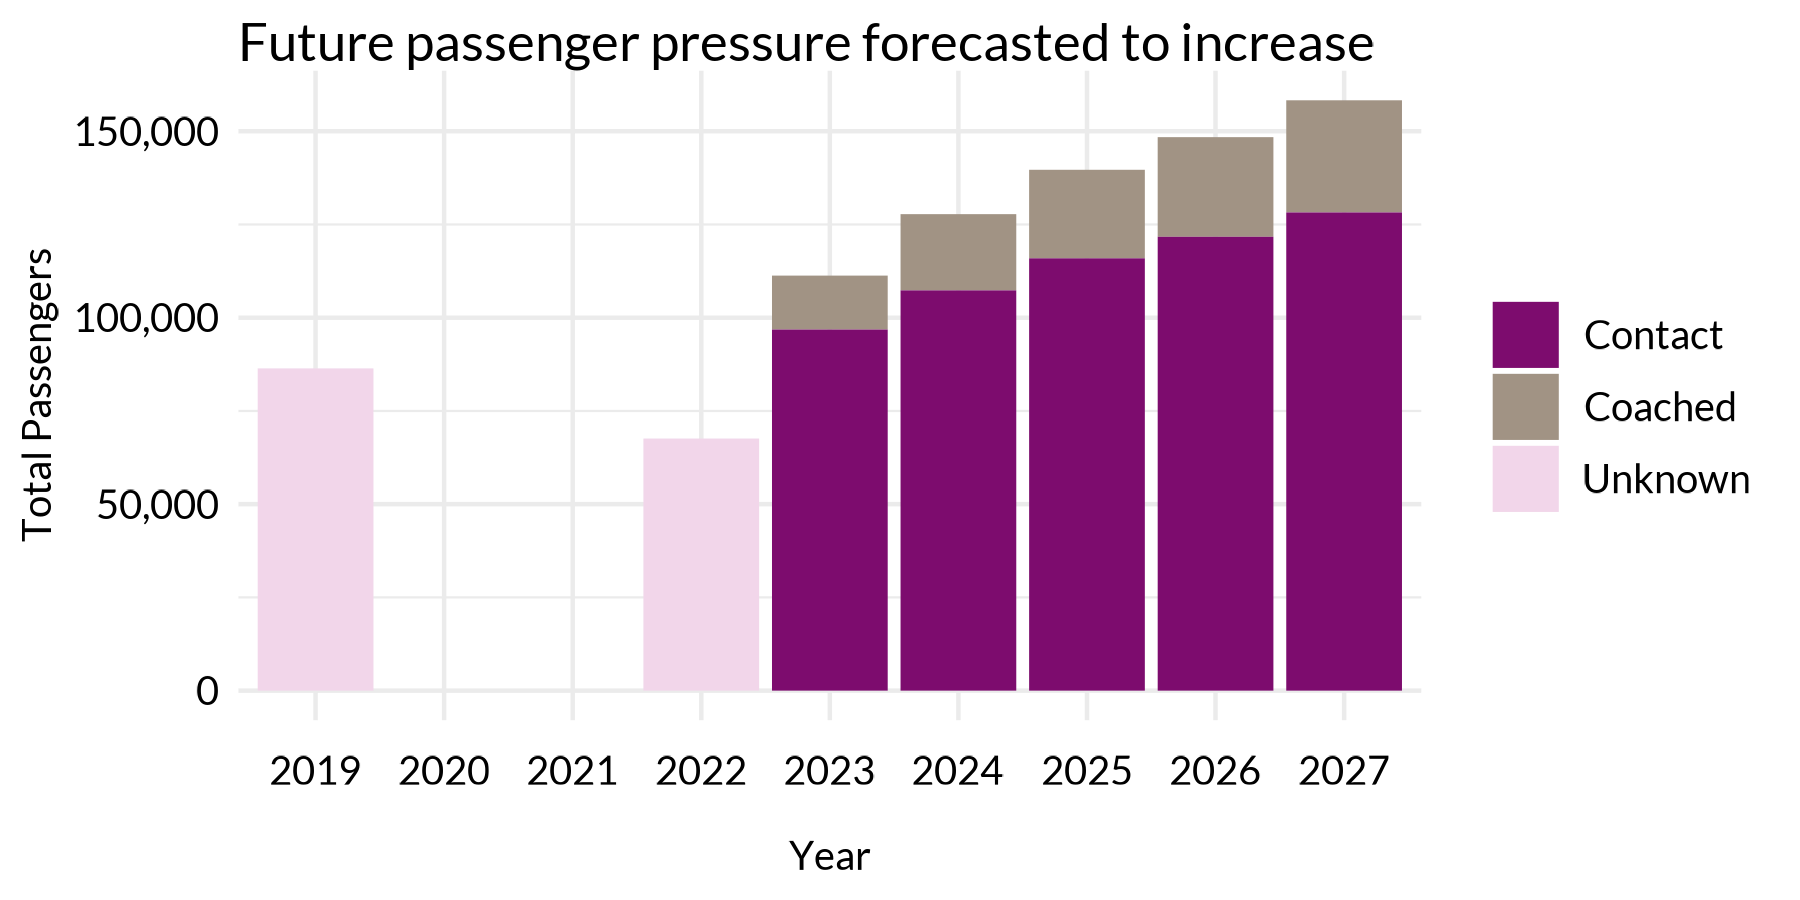
\includegraphics[width=0.8\textwidth]{figures/future_passenger_burden_fig.png}
     \caption{Anticipated future international contact/coached passenger arrivals in designated weeks over the next five years, alongside historical levels (note Covid-19 associated lows for 2020-2022). \bdnote{Are the histroic for non UK+ flights only?} \jbnote{Yes}} \label{fig:future_passenger_burden}
\end{figure}

\subsection{External Datasets} \label{sec:observed_arrivals_data}

\paragraph{eGate Utilisation}
The UK government's target for \gls{egate} usage among those eligible is 80\% \cite{UK_border_2025}, which was broadly met on a national level in 2019 and the first quarter of 2020. For airports in the North the uptake was consistently lower at around 70\% for the same period \cite{Inspection_eGates}. While there were no publicly available data for Edinburgh Airport, Glasgow Airport's uptake of around 60\% represents some of the lowest utilisation of \glspl{egate} nationwide \cite{Inspection_eGates}, and may serve as a reference/lower band due to its proximity.

\paragraph{Average Queue Time for eGates}
The average queue time at \glspl{egate} at UK airports for the financial years 2017-18, 2018-19, 2019-20 and Q1 2020 was six minutes and one second \cite{Inspection_eGates}. Stansted and Luton reported averages just below the three minute mark. Glasgow Airport's average waiting time at the \glspl{egate} was over 8.5 minutes. However, their calculation was based a shorter time period (December 2017, January 2018, and February 2019), and may therefore be unrepresentative \cite{Inspection_eGates}.


\paragraph{Historical Arrivals Data}
We accessed complementary historical historical flight arrivals data from the Edinburgh Airport Noise Lab \cite{noise_lab}. For these 83,652 passenger flight arrivals, spread Q1-4 for the years 2019 and 2022 (Table~\ref{tab:observed_arrivals_overview}), we were able to recover airport of origin, aircraft type (and therefore a proxy for passenger count), and scheduled vs. actual arrival time. We were not, however (unlike for anticipated future arrivals) able to recover coached vs. contact status (Figure~\ref{fig:future_passenger_burden}). We see this dataset, therefore, as useful for validating distributional assumptions around aircraft arrival times and passenger demographics. 


\begin{table}[!ht]
\caption{Historical datasets of Edinburgh Airport Arrivals. \bdnote{Need to add the other years here as well.} \jbnote{I have a cunnning plan for this.}}
\label{tab:observed_arrivals_overview}
\centering
\begin{tabular}{ccccc}
\hline
\multicolumn{1}{c}{\textbf{Dataset}} & \textbf{Year} & \textbf{Start Date} & \textbf{End Date} & \textbf{Number of Flights} \\ \hline
1  & 2019  & 01/01  & 31/12    &  51,669  \\
2  & 2022  & 01/01  & 31/12    &  31,983  \\
 \hline
\end{tabular}
\end{table}


Aircraft type and maximum passenger capacity were established by cross-linking with another publicly available dataset \cite{aircraft_capacity}. The average percentage of occupied seat for a given flight ranges from 86\% in 2019 for international flights in the UK \cite{loading_factor_national} to self-reported 91\% for a budget airline in 2022 \cite{loading_factor_ryanair}. This is called the \textit{load factor}.

\paragraph{Airport Classification}
We assume that the passenger nationality split depends on departure airport, and therefore group airports into the following categories: 
\begin{itemize}
    \item \textbf{UK+}: All airports in the United Kingdom (including Northern Ireland), the Crown Dependencies, and the Republic of Ireland.
    \item \textbf{EU+ hubs}: Hub airports in EU+. These are Amsterdam Schiphol (AMS), Atlanta International (ATL), Paris Charles de Gaulle (CDG), Dallas (DFW), Denver (DEN), Frankfurt (FRA), and Chicago O'Hare (ORD) \cite{mega_hubs}.
    \item \textbf{EU+ non-hubs}: Airports which are not hubs but are located in EU+.
    \item \textbf{Other hubs}: Hub airports outside of EU+. These are Dubai (DBX) and Istanbul (IST) \cite{mega_hubs}.
    \item \textbf{Other non-hubs}: Airports which are not hubs and are located outside of EU+.
\end{itemize}




\section{Passenger Processing Model}

    For all subsequent modelling we use a conceptual `passenger processing model' describing the steps an arriving international passenger experiences at Edinburgh Airport. Such a model is inherently a simplified view, but ideally chosen at a level of abstraction is nevertheless informative of real-world processes. The passenger processing model consist of three steps, which are outlined below and in subsequent sections:
\begin{enumerate}
    \item \textbf{Aircraft}: Aircraft with passengers on board arrive at Edinburgh Airport. The aircraft taxi to their parking positions and their doors are opened. \label{step:aircraft}
    \item \textbf{Route}: Passengers make their way from their aircraft to the immigration hall, either by walking to the building (contact) or via a bus (coached). \label{step:route}
    \item \textbf{Immigration}: Passengers queue in the immigration hall and are processed at the border, either by a \gls{bfo} at a desk or at an automated \gls{egate}. \label{step:immigration}
\end{enumerate}
 We visualise the flow of information through our processing model in Figure~\ref{fig:PPM_threesteps}. We start with a dataset of arriving flights and generate a dataset of passengers (\textit{Aircraft} step). In the \textit{Route} step these passengers are then brought from the aircraft to the immigration hall. Finally, in the \textit{Immigration} step they queue up and are subsequently processed at the border.

\begin{figure}[!ht]
    \centering
    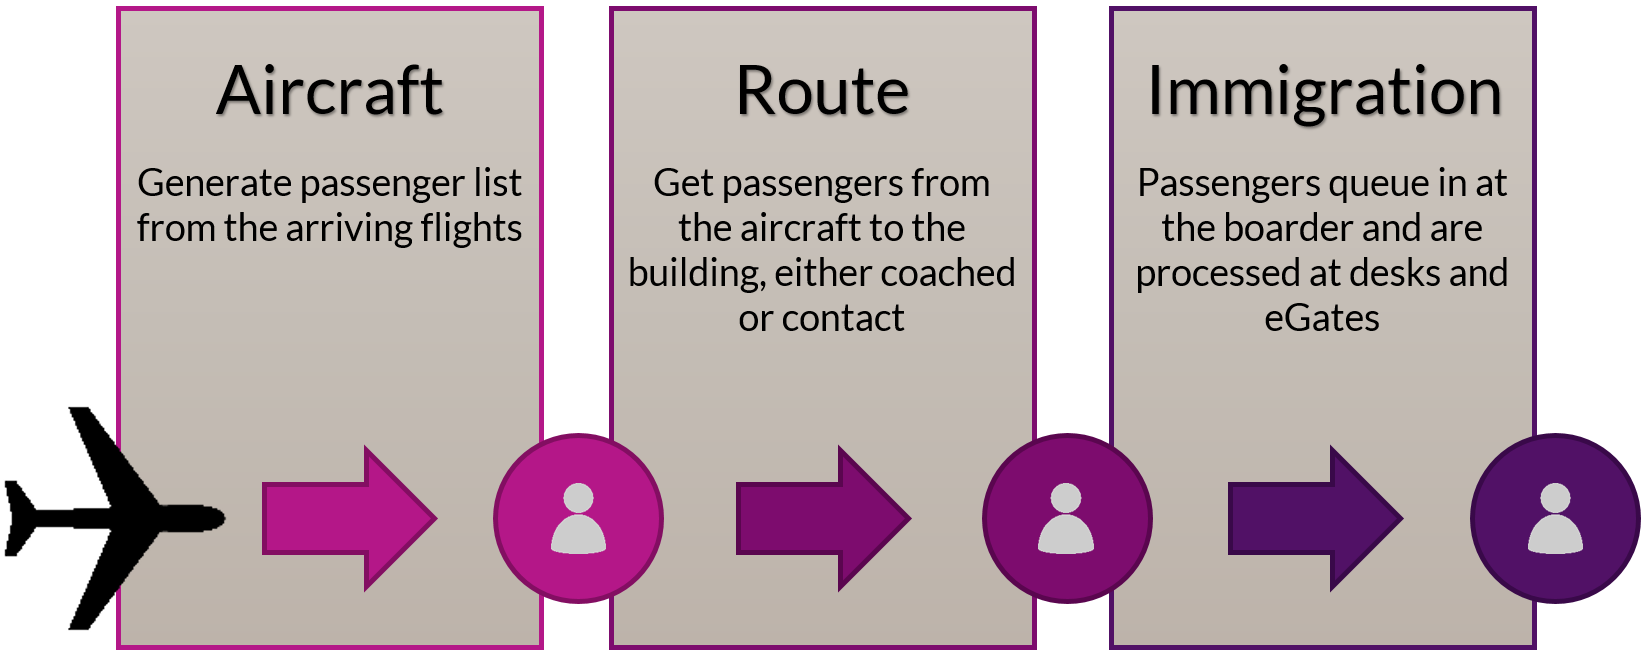
\includegraphics[width=0.7\textwidth]{figures/ThreeSteps.png}
     \caption{Three steps that make up the passenger processing model.  } \label{fig:PPM_threesteps}
\end{figure}

\subsection{Distributional Assumptions and Choices of Parameters}
% these are slightly different for competition and noise data

\subsubsection{Aircraft}

\paragraph{Departing Airport Classification}
The arrivals dataset provided by the modelling competition (Section~\ref{sec:future_arrivals_data}) does not contain information regarding the departing airport. As this is provided in the additional dataset (Section~\ref{sec:observed_arrivals_data}) we are able to randomly sample airport classifications for the competition dataset conditional on the number of passengers on the flight, for an approximate distributional match. 



% \paragraph{Number of Passengers}
% The competition dataset contains the number of passengers on board each flight. This information is not available for the additional historical data, but can be simulated with the aircraft type, its maximum capacity, and the load factor. \jbnote{Do we need to choose an overall load factor? Also slightly unsure if we'll ever actually ever need this simulated on historical data.} \bdnote{we use it indirectly to simulate an airport classification as the load factor goes into the historical quantiles. Could also be ignored.}

\paragraph{Coached vs. Contact}
The competition data gives an overall split of flights that are coached or contact for each year. As there was no additional information available we assume that the decision between coached or contact is independent of all flight characteristics, including passenger number. Anticipated future coached vs. contact splits are shown in Figure~\ref{fig:future_passenger_burden}, with coached arrivals continuing to form a minority, albeit an increasing one, of future aircraft arrivals. We explore the effects of non-independent occurrence of coached arrivals in Section~XX \jbnote{Robustness analysis I'd like to do: repeat whatever the main analysis pipeline is, with all coached in the biggest flights}.


\subsubsection{Route}

\paragraph{Bulk Profile} 
 Passengers  brought to the immigration hall coach arrive at the queue in rapid succession. We choose a XXX distribution  here.

\paragraph{Coach Availability}
For this analysis we assume sufficient coaches are always available to transport passengers from the aircraft to the airport building. While this might not be always the case, it provides us with a ``worst case'' scenario from the perspective of the immigration hall, which is most interesting for us. Any delay in passengers due to unavailability of coaches would smooth out peaks. \jbnote{I do think we should play with this though (only report if it's interesting.)} \bdnote{Would put a low piority on this right now.}


\subsubsection{Immigration}

\paragraph{Number of \glspl{egate} and Desks} There are currently 10 \glspl{egate} and 9 \gls{bfo}-staffed desks in use at Edinburgh Airport. In our analysis we simulate the effects of increased \gls{egate} construction.

\paragraph{eGate Eligibility} 
As only passengers from certain countries are can use \glspl{egate}, we make the percentage of passengers eligible for \glspl{egate} per aircraft dependent on the classification of the airport. For example, we assume that an aircraft from a hub is more likely to carry a variety of international passengers, of which fewer can use \glspl{egate} compared to a flight from a EU+ non-hub. \jbnote{This needs a lot of attention, in write up and in modelling approach.}

\paragraph{\gls{egate} Uptake and Failure Rate} 
Not all passengers who are eligible to use eGates choose to do so for a variety of reasons. We vary the percentage of \gls{egate} uptake between XX and XX. \jbnote{Is this varying randomly or systematically? If randomly, seems better just to pick a bad case.} 

\paragraph{eGate Failure Rate}
A small percentage of passengers who use an \gls{egate} fail to pass through it successfully. This is set to lie between XX and XX. \jbnote{As above.} \bdnote{hmm, maybe we just fix to something sensible? or do two cases: sensible and bad? Question: is "choosing a bad day" what they want? Do they want to know whta happens on average on a busy day or do they want the bad case avoided? given their SLAs I would say the former.}

\paragraph{Priority for failed \gls{egate} passengers}
Passengers who used an \gls{egate}, but failed to use it successfully, need to exit the \gls{egate} back into the immigration hall to complete their immigration at a staffed desk. They join a separate queue towards the desks, which is located next to the general desk queue. Whenever a desk can handle a new person, priority is given to the passenger from the failed \gls{egate} queue with a probability of XX to XX.

\paragraph{Capacity Split}

Which percentage of the hall capacity, overflow , and contingency is allocated to the desk queue. Varied to change the effect of queue length of contingency usage.



\section{Analysis}
\bdnote{this should get a better title (I gave it this title and still can't come up with anything better)}

\subsection{Methodology}
We explain how we simulate the airports they came from \\
describe any other simulation input needed, maybe different scenarios \\ 
be clear that this is (almost) just what they asked for  \\ Assumption: provided flights are all/mostly non-UKIE (compare to Noise dataset)



\subsection{Results}
include KPIs here, as well as some fancy plots



\section{Robustness Considerations}
relate to service level agreement \\
talk about working \glspl{egate}/break down of \glspl{egate}  \\
what if there are more non-UKIE flights  \\ 
need to also talk about the hall setup here?



\section{Discussion}
summary of the project and our approach \\
the number of contact spaces is fixed at the airport so if you want more flights you need to coach them (unless you want to undertake big building works) 

\subsection{Recommendation for Hall Layout}
we talk about the split of queue space and the mechanism queue space is allocated in the overflow hall \\
this is a nice bonus they hinted at in the description, so I think we should include some info here (could be less detailled)

\subsection{Recommendation for Total Number of eGates}
we need to put our foot down and come up with a final number \\ 
this number can be put into perspective by comparing it to the existing number of eGates at UK airports and funding to  deliver a programme to install up to 70 gates, which can be found here: \cite{Inspection_eGates} \\
mention that this is the number of \textbf{working} eGates at any time, the eGate doc by the government has numbers on how often they break down, cite those here

\subsection{Future Work}
all the assumptions we made \\
to include limitations \\
include edge cases, such as all gates closed for high risk flights (see Government doc on \glspl{egate}) \\
signange and direction need to be clear (hosts inccrease this and are important 6.28 \cite{Inspection_eGates})

{\footnotesize
\bibliography{report/references}}
% \bibliography{report/references.bib}

\end{document}